\section{Konvexe Hülle}
\subsection{Einleitung}
\begin{frame}
	\frametitle{{Konvexe Hülle}}
	\begin{block} {Definition}
	Die \textbf{konvexe Hülle} in einem d-dimensionalen Raum mit n-Punkten ist die kleinste konvexe Menge, die alle n Punkte enthält
	\end{block}
	\pause
	\textbf{Konvexe Mengen} sind geometrische Figuren, die alle Verbindungsstrecken zwischen paarweise verschiedenen Punkten enthalten.
	\pause	
	\begin{figure}
		\mbox{
			\subfigure[\tiny{konvex}]{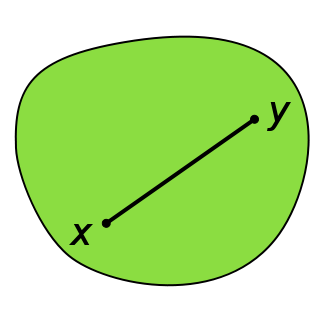
\includegraphics[width=.2\linewidth]{bilder/konvexeMenge.png}}\quad
			\hspace{1cm}
			\subfigure[\tiny{nicht konvex}]{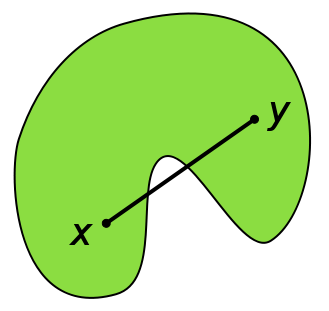
\includegraphics[width=.2\linewidth]{bilder/konvexeMenge2.png}}\quad
			\hspace{1cm}
			\subfigure[\tiny{{vollständiger Graph}}]{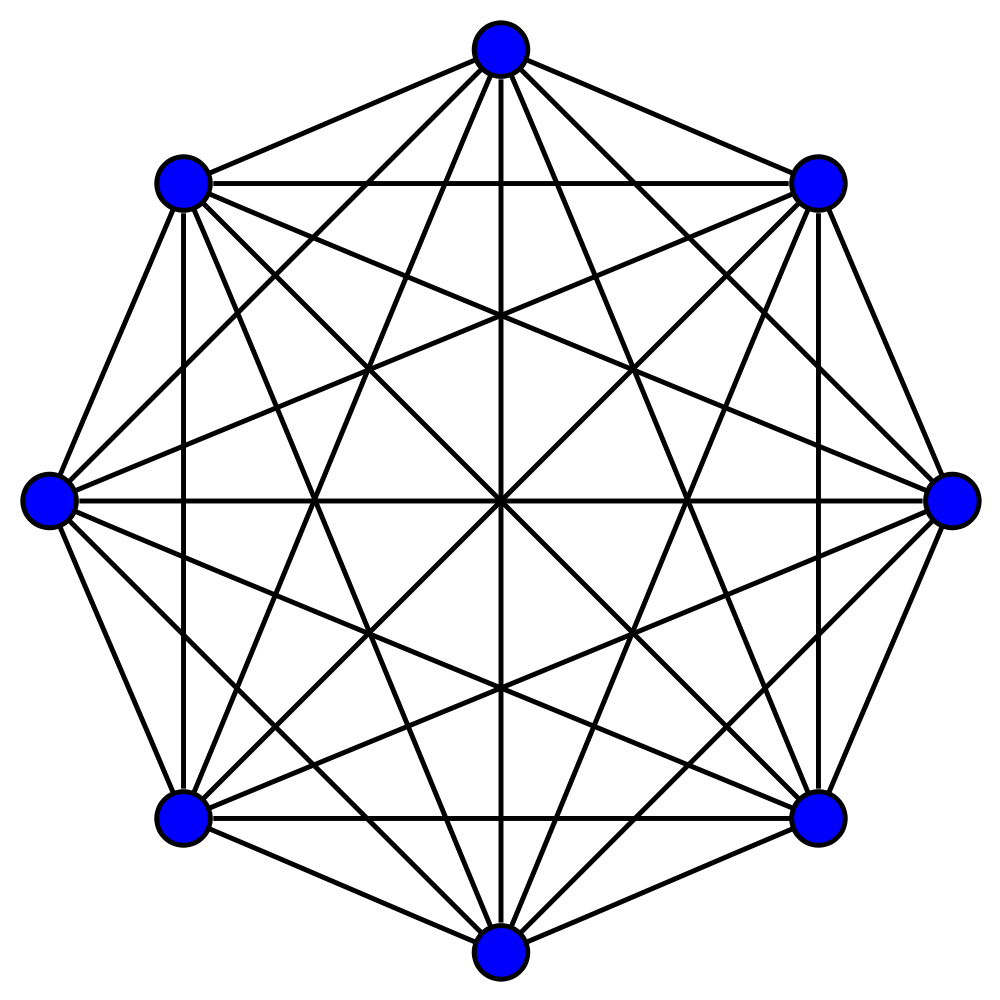
\includegraphics[width=.2\linewidth]{bilder/konvexeMenge3.png}}		
		}
	\end{figure}
	
\end{frame}
\subsection{Gift Wrapping}
\begin{frame}
	\frametitle{{Gift Wrapping}}
	sdfgsdfg
\end{frame}
\subsection{Graham Scan}
\begin{frame}
	\frametitle{{Graham Scan}}
	asdfasdf
\end{frame}